\begin{quote}
This is part 26 of Categories for Programmers. Previously:
\href{https://bartoszmilewski.com/2017/03/14/algebras-for-monads/}{Algebras
for Monads}. See the
\href{https://bartoszmilewski.com/2014/10/28/category-theory-for-programmers-the-preface/}{Table
of Contents}.
\end{quote}

There are many intuitions that we may attach to morphisms in a category,
but we can all agree that if there is a morphism from the object
\texttt{a} to the object \texttt{b} than the two objects are in some way
``related.'' A morphism is, in a sense, the proof of this relation. This
is clearly visible in any poset category, where a morphism \emph{is} a
relation. In general, there may be many ``proofs'' of the same relation
between two objects. These proofs form a set that we call the hom-set.
When we vary the objects, we get a mapping from pairs of objects to sets
of ``proofs.'' This mapping is functorial --- contravariant in the first
argument and covariant in the second. We can look at it as establishing
a global relationship between objects in the category. This relationship
is described by the hom-functor:

\begin{verbatim}
C(-, =) :: Cop × C -> Set
\end{verbatim}

In general, any functor like this may be interpreted as establishing a
relation between objects in a category. A relation may also involve two
different categories \emph{C} and \emph{D}. A functor, which describes
such a relation, has the following signature and is called a profunctor:

\begin{verbatim}
p :: Dop × C -> Set
\end{verbatim}

Mathematicians say that it's a profunctor from \texttt{C} to \texttt{D}
(notice the inversion), and use a slashed arrow as a symbol for it:

\begin{verbatim}
C ↛ D
\end{verbatim}

You may think of a profunctor as a \emph{proof-relevant relation}
between objects of \emph{C} and objects of \emph{D}, where the elements
of the set symbolize proofs of the relation. Whenever \texttt{p\ a\ b}
is empty, there is no relation between \texttt{a} and \texttt{b}. Keep
in mind that relations don't have to be symmetric.

Another useful intuition is the generalization of the idea that an
endofunctor is a container. A profunctor value of the type
\texttt{p\ a\ b} could then be considered a container of \texttt{b}s
that are keyed by elements of type \texttt{a}. In particular, an element
of the hom-profunctor is a function from \texttt{a} to \texttt{b}.

In Haskell, a profunctor is defined as a two-argument type constructor
\texttt{p} equipped with the method called \texttt{dimap}, which lifts a
pair of functions, the first going in the ``wrong'' direction:

\begin{verbatim}
class Profunctor p where dimap :: (c -> a) -> (b -> d) -> p a b -> p c d
\end{verbatim}

The functoriality of the profunctor tells us that if we have a proof
that \texttt{a} is related to \texttt{b}, then we get the proof that
\texttt{c} is related to \texttt{d}, as long as there is a morphism from
\texttt{c} to \texttt{a} and another from \texttt{b} to \texttt{d}. Or,
we can think of the first function as translating new keys to the old
keys, and the second function as modifying the contents of the
container.

For profunctors acting within one category, we can extract quite a lot
of information from diagonal elements of the type \texttt{p\ a\ a}. We
can prove that \texttt{b} is related to \texttt{c} as long as we have a
pair of morphisms \texttt{b-\textgreater{}a} and
\texttt{a-\textgreater{}c}. Even better, we can use a single morphism to
reach off-diagonal values. For instance, if we have a morphism
\texttt{f::a-\textgreater{}b}, we can lift the pair
\texttt{\textless{}f,\ idb\textgreater{}} to go from \texttt{p\ b\ b} to
\texttt{p\ a\ b}:

\begin{verbatim}
dimap f id pbb :: p a b
\end{verbatim}

Or we can lift the pair \texttt{\textless{}ida,\ f\textgreater{}} to go
from \texttt{p\ a\ a} to \texttt{p\ a\ b}:

\begin{verbatim}
dimap id f paa :: p a b
\end{verbatim}

\subsection{Dinatural Transformations}\label{dinatural-transformations}

Since profunctors are functors, we can define natural transformations
between them in the standard way. In many cases, though, it's enough to
define the mapping between diagonal elements of two profunctors. Such a
transformation is called a dinatural transformation, provided it
satisfies the commuting conditions that reflect the two ways we can
connect diagonal elements to non-diagonal ones. A dinatural
transformation between two profunctors \texttt{p} and \texttt{q}, which
are members of the functor category \texttt{{[}Cop\ ×\ C,\ Set{]}}, is a
family of morphisms:

\begin{verbatim}
αa :: p a a -> q a a
\end{verbatim}

for which the following diagram commutes, for any
\texttt{f::a-\textgreater{}b}:

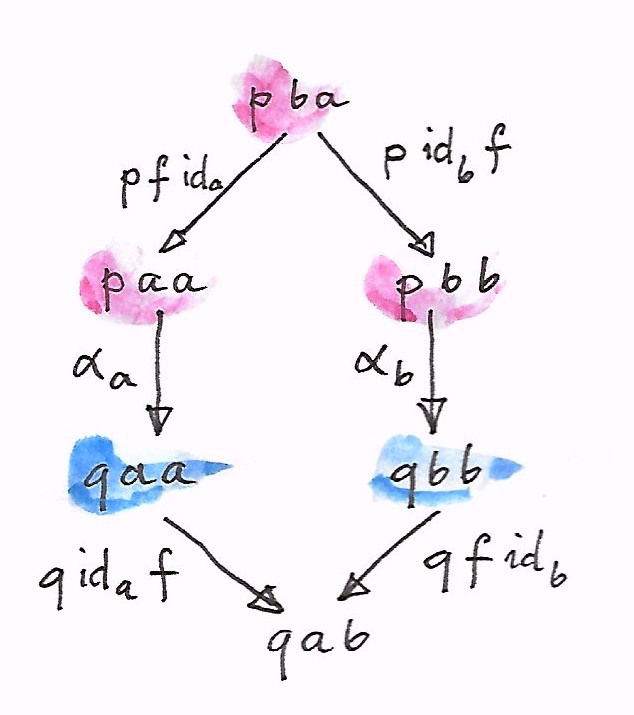
\includegraphics[width=2.77083in]{images/end.jpg}

Notice that this is strictly weaker than the naturality condition. If
\texttt{α} were a natural transformation in
\texttt{{[}Cop\ ×\ C,\ Set{]}}, the above diagram could be constructed
from two naturality squares and one functoriality condition (profunctor
\texttt{q} preserving composition):

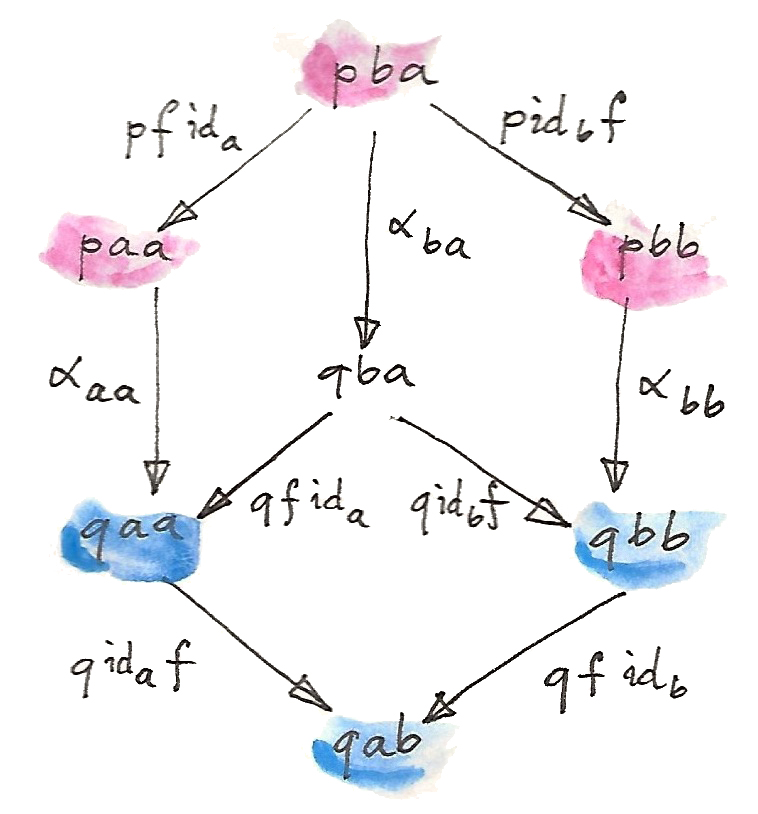
\includegraphics[width=3.36458in]{images/end-1.jpg}

Notice that a component of a natural transformation \texttt{α} in
\texttt{{[}Cop\ ×\ C,\ Set{]}} is indexed by a pair of objects
\texttt{α\ a\ b}. A dinatural transformation, on the other hand, is
indexed by one object, since it only maps diagonal elements of the
respective profunctors.

\subsection{Ends}\label{ends}

We are now ready to advance from ``algebra'' to what could be considered
the ``calculus'' of category theory. The calculus of ends (and coends)
borrows ideas and even some notation from traditional calculus. In
particular, the coend may be understood as an infinite sum or an
integral, whereas the end is similar to an infinite product. There is
even something that resembles the Dirac delta function.

An end is a generalization of a limit, with the functor replaced by a
profunctor. Instead of a cone, we have a wedge. The base of a wedge is
formed by diagonal elements of a profunctor \texttt{p}. The apex of the
wedge is an object (here, a set, since we are considering
\textbf{Set}-valued profunctors), and the sides are a family of
functions mapping the apex to the sets in the base. You may think of
this family as one polymorphic function --- a function that's
polymorphic in its return type:

\begin{verbatim}
α :: forall a . apex -> p a a
\end{verbatim}

Unlike in cones, within a wedge we don't have any functions that would
connect the vertices that form the base. However, as we've seen earlier,
given any morphism \texttt{f::a-\textgreater{}b} in \emph{C}, we can
connect both \texttt{p\ a\ a} and \texttt{p\ b\ b} to the common set
\texttt{p\ a\ b}. We therefore insist that the following diagram
commute:

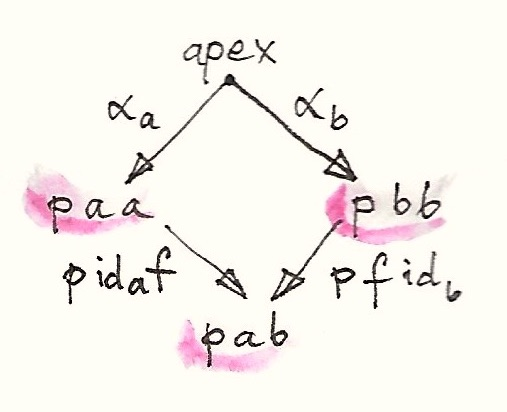
\includegraphics[width=2.69792in]{images/end-2.jpg}

This is called the wedge condition. It can be written as:

\begin{verbatim}
p ida f ∘ αa = p f idb ∘ αb
\end{verbatim}

Or, using Haskell notation:

\begin{verbatim}
dimap id f . alpha = dimap f id . alpha
\end{verbatim}

We can now proceed with the universal construction and define the end of
\texttt{p} as the uinversal wedge --- a set \texttt{e} together with a
family of functions \texttt{π} such that for any other wedge with the
apex \texttt{a} and a family \texttt{α} there is a unique function
\texttt{h::a-\textgreater{}e} that makes all triangles commute:

\begin{verbatim}
πa ∘ h = αa
\end{verbatim}

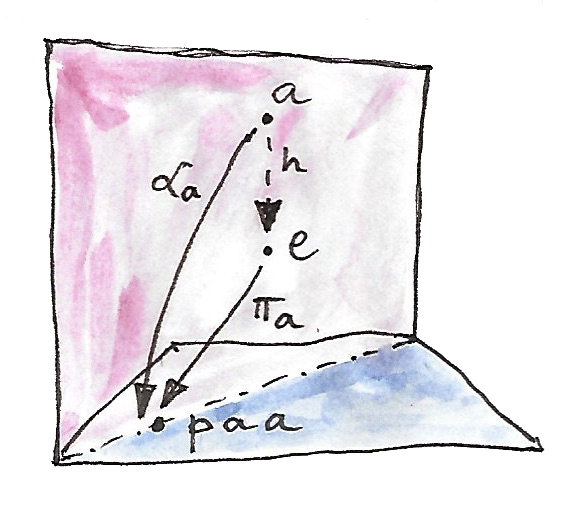
\includegraphics[width=2.73958in]{images/end-21.jpg}

The symbol for the end is the integral sign, with the ``integration
variable'' in the subscript position:

\begin{verbatim}
∫c p c c
\end{verbatim}

Components of \texttt{π} are called projection maps for the end:

\begin{verbatim}
πa :: ∫c p c c -> p a a
\end{verbatim}

Note that if \emph{C} is a discrete category (no morphisms other than
the identities) the end is just a global product of all diagonal entries
of \texttt{p} across the whole category \emph{C}. Later I'll show you
that, in the more general case, there is a relationship between the end
and this product through an equalizer.

In Haskell, the end formula translates directly to the universal
quantifier:

\begin{verbatim}
forall a. p a a
\end{verbatim}

Strictly speaking, this is just a product of all diagonal elements of
\texttt{p}, but the wedge condition is satisfied automatically due to
parametricity (I'll explain it in a
\href{https://bartoszmilewski.com/2017/04/11/profunctor-parametricity/}{separate
blog post}). For any function \texttt{f\ ::\ a\ -\textgreater{}\ b}, the
wedge condition reads:

\begin{verbatim}
dimap f id . pi = dimap id f . pi
\end{verbatim}

or, with type annotations:

\begin{verbatim}
dimap f idb . pib = dimap ida f . pia
\end{verbatim}

where both sides of the equation have the type:

\begin{verbatim}
Profunctor p => (forall c. p c c) -> p a b
\end{verbatim}

and \texttt{pi} is the polymorphic projection:

\begin{verbatim}
pi :: Profunctor p => forall c. (forall a. p a a) -> p c c pi e = e
\end{verbatim}

Here, type inference automatically picks the right component of
\texttt{e}.

Just as we were able to express the whole set of commutation conditions
for a cone as one natural transformation, likewise we can group all the
wedge conditions into one dinatural transformation. For that we need the
generalization of the constant functor \texttt{Δc} to a constant
profunctor that maps all pairs of objects to a single object \texttt{c},
and all pairs of morphisms to the identity morphism for this object. A
wedge is a dinatural transformation from that functor to the profunctor
\texttt{p}. Indeed, the dinaturality hexagon shrinks down to the wedge
diamond when we realize that \texttt{Δc} lifts all morphisms to one
identity function.

Ends can also be defined for target categories other than \textbf{Set},
but here we'll only consider \textbf{Set}-valued profunctors and their
ends.

\subsection{Ends as Equalizers}\label{ends-as-equalizers}

The commutation condition in the definition of the end can be written
using an equalizer. First, let's define two functions (I'm using Haskell
notation, because mathematical notation seems to be less user-friendly
in this case). These functions correspond to the two converging branches
of the wedge condition:

\begin{verbatim}
lambda :: Profunctor p => p a a -> (a -> b) -> p a b lambda paa f = dimap id f paa rho :: Profunctor p => p b b -> (a -> b) -> p a b rho pbb f = dimap f id pbb
\end{verbatim}

Both functions map diagonal elements of the profunctor \texttt{p} to
polymorphic functions of the type:

\begin{verbatim}
type ProdP p = forall a b. (a -> b) -> p a b
\end{verbatim}

These functions have different types. However, we can unify their types,
if we form one big product type, gathering together all diagonal
elements of \texttt{p}:

\begin{verbatim}
newtype DiaProd p = DiaProd (forall a. p a a)
\end{verbatim}

The functions \texttt{lambda} and \texttt{rho} induce two mappings from
this product type:

\begin{verbatim}
lambdaP :: Profunctor p => DiaProd p -> ProdP p lambdaP (DiaProd paa) = lambda paa rhoP :: Profunctor p => DiaProd p -> ProdP p rhoP (DiaProd paa) = rho paa
\end{verbatim}

The end of \texttt{p} is the equalizer of these two functions. Remember
that the equalizer picks the largest subset on which two functions are
equal. In this case it picks the subset of the product of all diagonal
elements for which the wedge diagrams commute.

\subsection{Natural Transformations as
Ends}\label{natural-transformations-as-ends}

The most important example of an end is the set of natural
transformations. A natural transformation between two functors
\texttt{F} and \texttt{G} is a family of morphisms picked from hom-sets
of the form \texttt{C(F\ a,\ G\ a)}. If it weren't for the naturality
condition, the set of natural transformations would be just the product
of all these hom-sets. In fact, in Haskell, it is:

\begin{verbatim}
forall a. f a -> g a
\end{verbatim}

The reason it works in Haskell is because naturality follows from
parametricity. Outside of Haskell, though, not all diagonal sections
across such hom-sets will yield natural transformations. But notice that
the mapping:

\begin{verbatim}
<a, b> -> C(F a, G b)
\end{verbatim}

is a profunctor, so it makes sense to study its end. This is the wedge
condition:

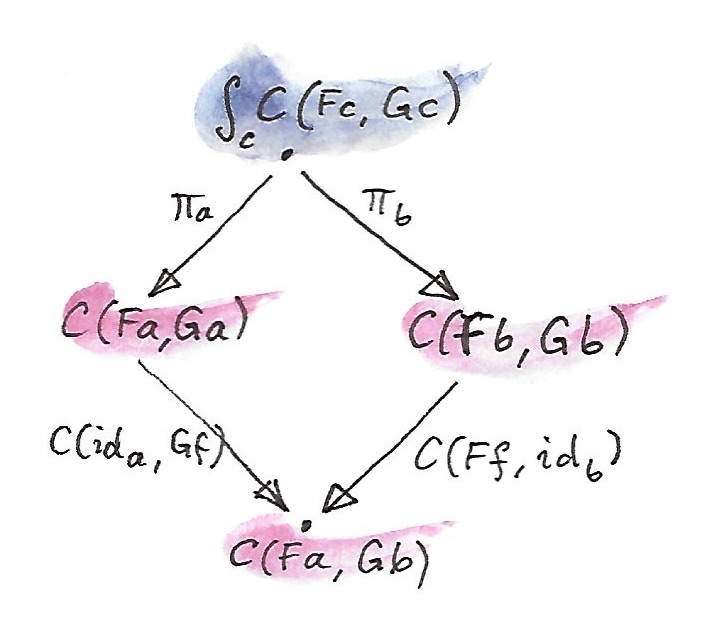
\includegraphics[width=3.12500in]{images/end1.jpg}

Let's just pick one element from the set \texttt{∫c\ C(F\ c,\ G\ c)}.
The two projections will map this element to two components of a
particular transformation, let's call them:

\begin{verbatim}
τa :: F a -> G a τb :: F b -> G b
\end{verbatim}

In the left branch, we lift a pair of morphisms
\texttt{\textless{}ida,\ G\ f\textgreater{}} using the hom-functor. You
may recall that such lifting is implemented as simultaneous pre- and
post-composition. When acting on \texttt{τa} the lifted pair gives us:

\begin{verbatim}
G f ∘ τa ∘ ida
\end{verbatim}

The other branch of the diagram gives us:

\begin{verbatim}
idb ∘ τb ∘ F f
\end{verbatim}

Their equality, demanded by the wedge condition, is nothing but the
naturality condition for \texttt{τ}.

\subsection{Coends}\label{coends}

As expected, the dual to an end is called a coend. It is constructed
from a dual to a wedge called a cowedge (pronounced co-wedge, not
cow-edge).

\hypertarget{attachment_8533}{}
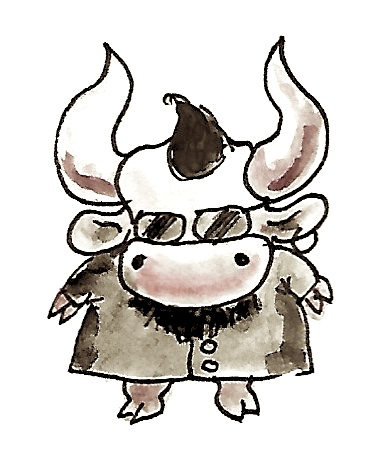
\includegraphics[width=1.82292in]{images/end-31.jpg}

\emph{An edgy cow?}

The symbol for a coend is the integral sign with the ``integration
variable'' in the superscript position:

\begin{verbatim}
∫ c p c c
\end{verbatim}

Just like the end is related to a product, the coend is related to a
coproduct, or a sum (in this respect, it resembles an integral, which is
a limit of a sum). Rather than having projections, we have injections
going from the diagonal elements of the profunctor down to the coend. If
it weren't for the cowedge conditions, we could say that the coend of
the profunctor \texttt{p} is either \texttt{p\ a\ a}, or
\texttt{p\ b\ b}, or \texttt{p\ c\ c}, and so on. Or we could say that
there exists such an \texttt{a} for which the coend is just the set
\texttt{p\ a\ a}. The universal quantifier that we used in the
definition of the end turns into an existential quantifier for the
coend.

This is why, in pseudo-Haskell, we would define the coend as:

\begin{verbatim}
exists a. p a a
\end{verbatim}

The standard way of encoding existential quantifiers in Haskell is to
use universally quantified data constructors. We can thus define:

\begin{verbatim}
data Coend p = forall a. Coend (p a a)
\end{verbatim}

The logic behind this is that it should be possible to construct a coend
using a value of any of the family of types \texttt{p\ a\ a}, no matter
what \texttt{a} we chose.

Just like an end can be defined using an equalizer, a coend can be
described using a \emph{coequalizer}. All the cowedge conditions can be
summarized by taking one gigantic coproduct of \texttt{p\ a\ b} for all
possible functions \texttt{b-\textgreater{}a}. In Haskell, that would be
expressed as an existential type:

\begin{verbatim}
data SumP p = forall a b. SumP (b -> a) (p a b)
\end{verbatim}

There are two ways of evaluating this sum type, by lifting the function
using \texttt{dimap} and applying it to the profunctor \texttt{p}:

\begin{verbatim}
lambda, rho :: Profunctor p => SumP p -> DiagSum p lambda (SumP f pab) = DiagSum (dimap f id pab) rho (SumP f pab) = DiagSum (dimap id f pab)
\end{verbatim}

where \texttt{DiagSum} is the sum of diagonal elements of \texttt{p}:

\begin{verbatim}
data DiagSum p = forall a. DiagSum (p a a)
\end{verbatim}

The coequalizer of these two functions is the coend. A coequilizer is
obtained from \texttt{DiagSum\ p} by identifying values that are
obtained by applying \texttt{lambda} or \texttt{rho} to the same
argument. Here, the argument is a pair consisting of a function
\texttt{b-\textgreater{}a} and an element of \texttt{p\ a\ b}. The
application of \texttt{lambda} and \texttt{rho} produces two potentially
different values of the type \texttt{DiagSum\ p}. In the coend, these
two values are identified, making the cowedge condition automatically
satisfied.

The process of identification of related elements in a set is formally
known as taking a quotient. To define a quotient we need an
\emph{equivalence relation} \texttt{\textasciitilde{}}, a relation that
is reflexive, symmetric, and transitive:

\begin{verbatim}
a ~ a if a ~ b then b ~ a if a ~ b and b ~ c then a ~ c
\end{verbatim}

Such a relation splits the set into equivalence classes. Each class
consists of elements that are related to each other. We form a quotient
set by picking one representative from each class. A classic example is
the definition of rational numbers as pairs of whole numbers with the
following equivalence relation:

\begin{verbatim}
(a, b) ~ (c, d) iff a * d = b * c
\end{verbatim}

It's easy to check that this is an equivalence relation. A pair
\texttt{(a,\ b)} is interpreted as a fraction \texttt{a/b}, and
fractions that have a common divisor are identified. A rational number
is an equivalence class of such fractions.

You might recall from our earlier discussion of limits and colimits that
the hom-functor is continuous, that is, it preserves limits. Dually, the
contravariant hom-functor turns colimits into limits. These properties
can be generalized to ends and coends, which are a generalization of
limits and colimits, respectively. In particular, we get a very useful
identity for converting coends to ends:

\begin{verbatim}
Set(∫ x p x x, c) ≅ ∫x Set(p x x, c)
\end{verbatim}

Let's have a look at it in pseudo-Haskell:

\begin{verbatim}
(exists x. p x x) -> c ≅ forall x. p x x -> c
\end{verbatim}

It tells us that a function that takes an existential type is equivalent
to a polymorphic function. This makes perfect sense, because such a
function must be prepared to handle any one of the types that may be
encoded in the existential type. It's the same principle that tells us
that a function that accepts a sum type must be implemented as a case
statement, with a tuple of handlers, one for every type present in the
sum. Here, the sum type is replaced by a coend, and a family of handlers
becomes an end, or a polymorphic function.

\subsection{Ninja Yoneda Lemma}\label{ninja-yoneda-lemma}

The set of natural transformations that appears in the Yoneda lemma may
be encoded using an end, resulting in the following formulation:

\begin{verbatim}
∫z Set(C(a, z), F z) ≅ F a
\end{verbatim}

There is also a dual formula:

\begin{verbatim}
∫ z C(a, z) × F z ≅ F a
\end{verbatim}

This identity is strongly reminiscent of the formula for the Dirac delta
function (a function \texttt{δ(a\ -\ z)}, or rather a distribution, that
has an infinite peak at \texttt{a\ =\ z}). Here, the hom-functor plays
the role of the delta function.

Together these two identities are sometimes called the Ninja Yoneda
lemma.

To prove the second formula, we will use the consequence of the Yoneda
embedding, which states that two objects are isomorphic if and only if
their hom-functors are isomorphic. In other words \texttt{a\ ≅\ b} if
and only if there is a natural transformation of the type:

\begin{verbatim}
[C, Set](C(a, -), C(b, =))
\end{verbatim}

that is an isomorphism.

We start by inserting the left-hand side of the identity we want to
prove inside a hom-functor that's going to some arbitrary object
\texttt{c}:

\begin{verbatim}
Set(∫ z C(a, z) × F z, c)
\end{verbatim}

Using the continuity argument, we can replace the coend with the end:

\begin{verbatim}
∫z Set(C(a, z) × F z, c)
\end{verbatim}

We can now take advantage of the adjunction between the product and the
exponential:

\begin{verbatim}
∫z Set(C(a, z), c(F z))
\end{verbatim}

We can ``perform the integration'' by using the Yoneda lemma to get:

\begin{verbatim}
c(F a)
\end{verbatim}

This exponential object is isomorphic to the hom-set:

\begin{verbatim}
Set(F a, c)
\end{verbatim}

Finally, we take advantage of the Yoneda embedding to arrive at the
isomorphism:

\begin{verbatim}
∫ z C(a, z) × F z ≅ F a
\end{verbatim}

\subsection{Profunctor Composition}\label{profunctor-composition}

Let's explore further the idea that a profunctor describes a relation
--- more precisely, a proof-relevant relation, meaning that the set
\texttt{p\ a\ b} represents the set of proofs that \texttt{a} is related
to \texttt{b}. If we have two relations \texttt{p} and \texttt{q} we can
try to compose them. We'll say that \texttt{a} is related to \texttt{b}
through the composition of \texttt{q} after \texttt{p} if there exist an
intermediary object \texttt{c} such that both \texttt{q\ b\ c} and
\texttt{p\ c\ a} are non-empty. The proofs of this new relation are all
pairs of proofs of individual relations. Therefore, with the
understanding that the existential quantifier corresponds to a coend,
and the cartesian product of two sets corresponds to ``pairs of
proofs,'' we can define composition of profunctors using the following
formula:

\begin{verbatim}
(q ∘ p) a b = ∫ c p c a × q b c
\end{verbatim}

Here's the equivalent Haskell definition from
\texttt{Data.Profunctor.Composition}, after some renaming:

\begin{verbatim}
data Procompose q p a b where Procompose :: q a c -> p c b -> Procompose q p a b 
\end{verbatim}

This is using generalized algebraic data type, or GADT syntax, in which
a free type variable (here \texttt{c}) is automatically existentially
quanitified. The (uncurried) data constructor \texttt{Procompose} is
thus equivalent to:

\begin{verbatim}
exists c. (q a c, p c b)
\end{verbatim}

The unit of so defined composition is the hom-functor --- this
immediately follows from the Ninja Yoneda lemma. It makes sense,
therefore, to ask the question if there is a category in which
profunctors serve as morphisms. The answer is positive, with the caveat
that both associativity and identity laws for profunctor composition
hold only up to natural isomorphism. Such a category, where laws are
valid up to isomorphism, is called a bicategory (which is more general
than a 2-category). So we have a bicategory \textbf{Prof}, in which
objects are categories, morphisms are profunctors, and morphisms between
morphisms (a.k.a., two-cells) are natural transformations. In fact, one
can go even further, because beside profunctors, we also have regular
functors as morphisms between categories. A category which has two types
of morphisms is called a double category.

Profunctors play an important role in the Haskell lens library and in
the arrow library.

\subsection{Challenge}\label{challenge}

\begin{enumerate}
\tightlist
\item
  Write explicitly the cowedge condition for a coend.
\end{enumerate}

Next: \href{https://bartoszmilewski.com/2017/04/17/kan-extensions/}{Kan
extensions}.
